\documentclass[../main.tex]{subfiles}

\begin{document}
\subsection{Friction Wheel Slip} \label{frictionSlip}
\begin{figure}[H]
	\centering
	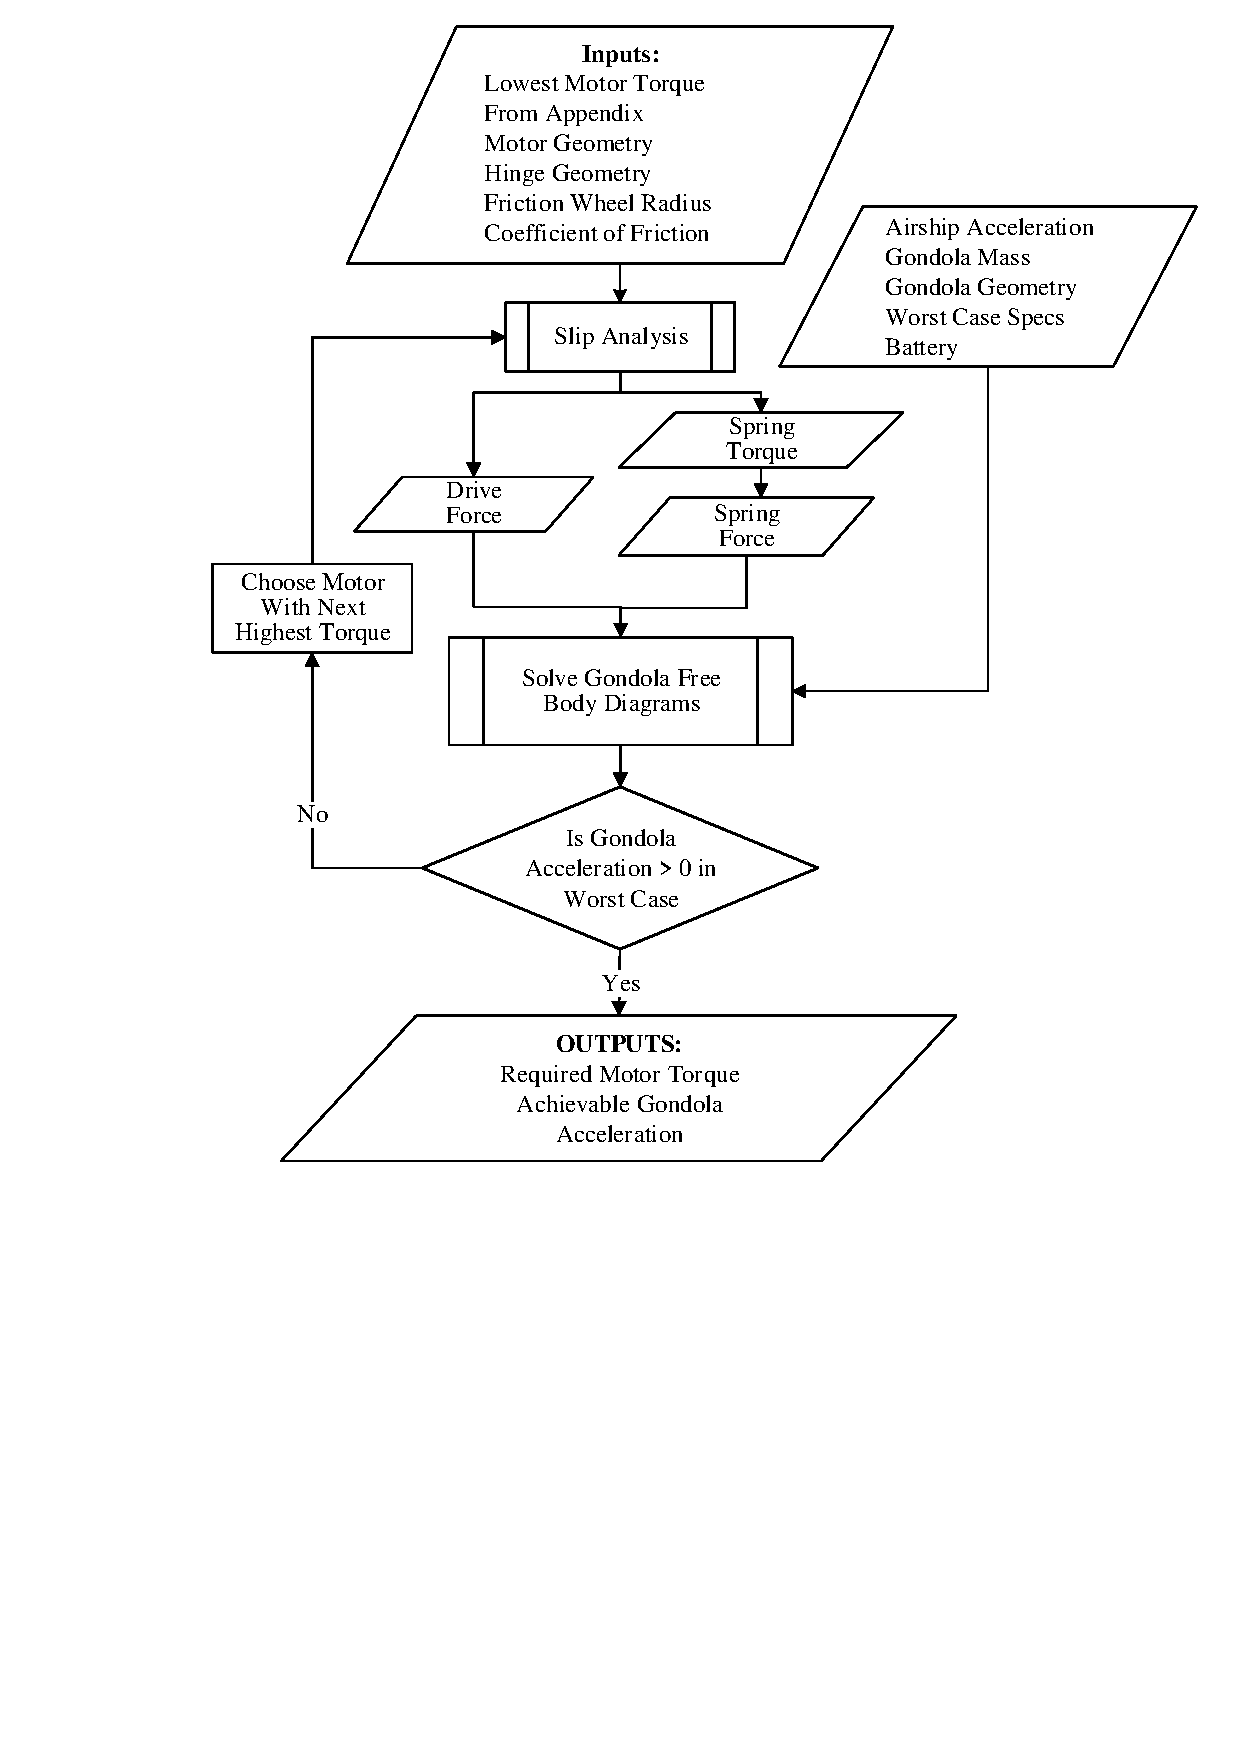
\includegraphics[width=.9\linewidth]{img/paramaterization/fricWheelSlip.pdf}
	\caption{Parametrization Outline for the Friction Wheel Slip}
	\label{fig:frictionWheelParametrization}
\end{figure}

The friction wheel slip analysis, calculates the required motor torque in order to allow for the gondola to move in a worst case scenario, and then calculates the motor hinge spring torque that will generate a large enough normal force to prevent slip of the friction wheel. The inputs required for the analysis are the geometry of the friction wheel, the motor, the hinge, the gondola, as well as the material properties of the friction wheel, the mass of each gondola car, the maximum achievable thruster acceleration and the loading conditions specific to the worst case scenario. \\

The friction wheel slip analysis, calculates the required motor torque in order to allow for the gondola to move in a worst case scenario, and then calculates the motor hinge spring torque that will generate a large enough normal force to prevent slip of the friction wheel. The inputs required for the analysis are the geometry of the friction wheel, the motor, the hinge, the gondola, as well as the material properties of the friction wheel, the mass of each gondola car, the maximum achievable acceleration as a result of the thrusters and the loading conditions specific to the worst case scenario. \\


Parameters that will not change through out the gondola analysis include, the geometry of the motor, this is because different torques can be achieved with the same geometry by modifying the gearing. See Appendix \ref{FrictionMotor}. The geometry of the hinge will not change as it is aluminium and the forces applied to it are minimal. The components inside of the gondola which include the R.F transmitter, the BESC and the battery will not be changing. Calculations for required power and run time are done in APPENDIX********* show that regardless of motor gearing, power requirements are easily met and the limiting factor for flight time will be the thruster batteries. As a result the geometry of the main frame of the gondola (length, width, and height) will not be parameterized and the weights of the gondola will remains approximately the same. \\

The analysis first assumes a motor torque. With this torque the code computes the spring torque such that $F_{spring} = F_{Nfric}$, which ensures the friction wheel will not slip. For the purpose of this analysis, the friction wheel and shaft interface are considered without slip, and the set screw is assumed to not fail as it will be metal interfacing with plastic.

\begin{equation}
F_{spring} = F_{Nfric} = \frac{F_{fFric}}{\mu} = \frac{T_w}{r_{Fw}\cdot{}\mu}
\end{equation}
\begin{equation}
F_{spring} = \frac{T_{spring}}{L_{hs}+L_{sw}}
\end{equation}
\begin{equation}
\frac{T_{spring}}{[L_{hs}+L_{sw}]} = \frac{T_w}{r_{Fw}\cdot{}\mu}
\end{equation}

The relation for the minimum necessary spring torque is multiplied by a factor of 1.5 in order to account for any neglected external factors.

\begin{equation}
T_{spring} = \frac{T_w\cdot{}[L_{hs}+L_{sw}]}{r{F_w}\cdot{}\mu}\cdot{}1.5
\end{equation}

Based on the assumed torque and the spring force, the acceleration of the gondola in the worst case scenario explained in SECTION????, and FIGURE ????? The acceleration of the gondola is calculated, The forces acting 
The following equations \ref{Fxgondtw} to \ref{Fzgondtw} are the sum of forces acting on the gondola in the coordinate system defined by the plane of the surface of the rear gondola car. As a result most of the forces and reactions acting on the front gondola need to be rotated according to the angle of the hinge, $\Theta$ is the angle between the gondolas. Similarly $\phi$ is the pitch angle of the airship and $\beta$ is the angle at which the acceleration due to thrust is acting. The reactions are on the left of the equal sign and the known forces acting on the gondola are to the right of the equal sign. 
\begin{multline} \label{Fxgondtw}
\Sigma F_{x} : (m_{1}+m_{2}) a_{x} + F_{NB3_{x}} + F_{NB4_{x}} =\\ \sin(\phi) (m_{1} + m_2)g + F_{Drive} + \cos (\Theta) F_{Drive} + \cos(\beta) (m_1+m_2) a_{Thrust} + \frac{\sqrt{2}}{2} sin(\Theta) F_{Spring}
\end{multline}
\begin{flalign} \label{Fygondtw}
\hspace{12pt}\Sigma F_{y} : F_{NB1_{y}} - F_{NB2_{y}} - F_{NB3_{y}} + F_{NB4_{y}} = \frac{\sqrt{2}}{2} F_{Spring} -\frac{\sqrt{2}}{2} F_{Spring} &&
\end{flalign}
\begin{multline} \label{Fzgondtw}
\Sigma F_{z} : F_{NB1_{z}} + F_{NB2_{z}} + F_{NB3_{z}} + F_{NB4_{z}} =\\ \cos(\phi) (m_{1} + m_2)g - \frac{\sqrt{2}}{2} cos(\Theta) F_{Spring} -\frac{\sqrt{2}}{2} F_{Spring} + \sin(\beta) (m_1+m_2) a_{Thrust}+\sin (\Theta) F_{Drive}
\end{multline}

Force solver ??? is used to solve these equations while making some assumptions based on the reactions. All of the $F_{NB}$ the normal forces between the bearings and the keel. since the contact surface is at 45\textdegree between the XY and XZ planes, the magnitudes of the forces acting in the z and y directions must be equal. 
\begin{align}
\label{eqn:scenario2start}
	 F_{NB1_{z}} &= - F_{NB1_{y}} \\
	 F_{NB2_{z}} &= F_{NB2_{y}} 
\end{align}

For the bearings on the front gondola as a result of the  angle between gondolas, there will also be a force acting in the x direction such that 
\begin{align}
F_{NB3_{x}} &= -\tan(\Theta) F_{NB3_{z}}\\ 
F_{NB4_{x}} &= -\tan(\Theta) F_{NB4_{z}}\\
F_{NB3_{y}} &= -\frac{F_{NB3_{z}}}{\cos(\Theta)} \\ F_{NB4_{y}} &= \frac{F_{NB4_{z}}}{\cos(\Theta)} \label{eqn:scenario2end}
\end{align}

The above equations from \ref{eqn:scenario2start} to \ref{eqn:scenario2end} are all encompassed by the switch case, scenario 2, in the Force Solver Code????. 
\end{document}